\begin{frame}
\frametitle{\small Состояние проблемы и основные трудности в предметной области}
\footnotesize
\vfill
3 стандартных подхода для решения задачи распознавания:
\vfill
\begin{itemize}
	\item \textbf{скрытые марковские модели} - хорошо распознают слитную речь,\\ но нужны модели языка и \underline{плохо работает в шумах} ($\sim 50\%$ ошибок)
	\item \textbf{сравнение с эталоном} - простой метод для распознавания отдельных слов, но только для ограниченного словаря
	\item \textbf{нейронные сети} - показывают лучшие результаты в последние годы, но долго обучаются и обычно нужна большая обучающая выборка
\end{itemize}
\vfill
Текущие значения доли неправильных распознаваний:
\vfill
\begin{itemize} 
	\item кабина пилота на самолётах Eurofighter Typhoon и Lockheed Martin F-16A и F-35: 10~\% для словаря 100--300 слов
	\item голосовой ввод Google: 23~\%~в~2013 году $\rightarrow$ 8~\%~в~2015 году $\rightarrow$\\$\rightarrow$ 4.9~\%~в~2017 году
	\item распознавание записей человеком: 0.1~\%~для~цифр, 1.6~\%~для~букв, 1~\%~предложения, 2~\%~бессмысленный~набор~слов, 4~\%~телефонные~разговоры
\end{itemize}
\vfill
\end{frame}

\begin{frame}
\frametitle{\normalsize Цель исследования и практическая значимость}
\footnotesize
\vfill
\textbf{Цель исследования:}
обеспечение повышения вероятности правильных распознаваний и снижение влияния акустических шумов, путём разработки алгоритмов распознавания команд речевого интерфейса кабины пилота
\vfill
\textbf{Особенности речевого интерфейса кабины пилота:}
\\
{\scriptsize
(дополнительный канал ввода для систем, некритичных для безопасности полёта)
}
\begin{itemize}
	\setlength\topsep{0pt}
	\setlength\partopsep{0pt}
	\item распознавание ограниченного словаря, состоящего из слов или фраз
	\item необходимость автономной системы
	\item высокое быстродействие для работы в режиме реального времени
	\item высокая вероятность правильных распознаваний
	\item устойчивость к акустическим шумам в кабине пилота
	%\item дикторонезависимость (необязательное условие)
\end{itemize}
\vfill
\textbf{Практическая значимость:} результаты могут быть использованы в ходе разработки алгоритмического обеспечения речевого интерфейса кабины пилота для управления бортовым оборудованием современных самолётов, \underline{например}: отображение информации, выбор частоты, прокладка маршрута, система опознавания, управление датчиками, запрос запаса топлива
\vfill
\end{frame}

\begin{frame}
\frametitle{\normalsize Научная новизна, объект и предмет исследования}
\footnotesize
\vfill
\textbf{Научная новизна} заключается в разработке совокупности алгоритмов, обеспечивающих повышение вероятности правильных распознаваний команд речевого интерфейса кабины пилота:
\vfill
\begin{itemize}
	\scriptsize
	\item алгоритм разбиения речевых команд на фонетически однородные части на основе модифицированного метода динамического программирования;
	\item алгоритм оптимизации эталонов на основе метода главных компонент;
	\item алгоритм оптимизации размерности параметрических портретов с использованием полиномов Чебышёва;
	\item алгоритм распознавания команд по нескольким эталонам с использование байесовского подхода и метода комитетов;
	\item алгоритм распознавания команд свёрточными нейронными сетями, способных обучаться на выборках малого размера.
\end{itemize}
\vfill
\textbf{Объект исследования:} в данной работе в качестве объекта исследования рассматриваются речевые команды
\vfill
\textbf{Предмет исследования:} методы и алгоритмы распознавания речевых команд являются предметами исследования в данной работе
\vfill
\end{frame}

\begin{frame}
\frametitle{Положения, выносимые на защиту}
\vfill
\begin{enumerate}
	\footnotesize
	\item \textit{Алгоритм разбиения речевых команд на фонетически однородные части}.
	Отличается от существующих применением модифицированного метода динамического программирования.
	\item \textit{Алгоритм оптимизации эталонов.}
	Отличается от существующих тем, что искомый эталон формируется как линейная комбинация главных компонент, оптимизирующая заданный критерий качества.
	\item \textit{Алгоритм оптимизации размерности параметрических портретов.}
	Отличается выделением наиболее значимых составляющих с использованием полиномов Чебышёва.
	\item \textit{Алгоритм распознавания команд по нескольким эталонам.}
	Отличается применением последовательного оценивания с расчётом апостериорных байесовских вероятностей.
	\item \textit{Алгоритм распознавания команд свёрточными нейронными сетями глубокого обучения.}
	Отличается от существующих обучением на выборке малого размера.
\end{enumerate}
\vfill
\end{frame}

\begin{frame}
\frametitle{Статьи и конференции}
\footnotesize
\vfill
\textbf{4 статьи}: 3 ВАК, 2 Scopus и Web of Science
\begin{enumerate}
	\scriptsize
	\item "Автоматическое выделение фонетически однородных участков в словах естественного языка на основе многопараметрической оптимизации"\
	в журнале
	<<Известия Российской академии наук. Теория и системы управления>>
	\item "Разработка алгоритма синтеза оптимальных эталонов на основе метода главных компонент"\
	в журнале
	<<Cloud of science>>
	\item "Использование нескольких эталонов при распознавании речи: формула Байеса и метод комитетов"\
	в журнале
	<<Вестник компьютерных и информационных технологий>>
	\item "Optimal pattern synthesis for speech recognition based on principal component analysis"\
	в журнале
	<<IOP Conference Series: Materials Science and Engineering>>
\end{enumerate}
\vfill
\textbf{9 выступлений на конференциях}: \\
Международный аэрокосмический конгресс IAC'15 и IAC'18;
XII и XIII Научные чтения по авиации посвящённые памяти Н.Е. Жуковского;
Авиационные системы в XXI веке 2016;
CMTAI 2016;
Эрго-2016: Человеческий фактор в сложных технических системах и средах;
Навигация, наведение и управление летательными аппаратами 2017;
Моделирование авиационных систем 2018
\vfill
\end{frame}

%%%%%%%%%%%%%%%%%%%%%%%%%%%%%%

\begin{frame}
\frametitle{Тестовая база речевых данных}
\footnotesize
\vfill
Для реализации поставленных задач была записана база речевых команд, часто применяемых в качестве управляющих в кабине пилота:
\scriptsize
\vfill
\begin{itemize}
	\item 20 слов (10 дикторов по 30 записей каждого слова): {\tiny ПИЛОТАЖ, МАСШТАБ, НАВИГАЦИЯ, ТЫСЯЧА, МЕНЬШЕ, ДВА, ДВАДЦАТЬ, ВЗЛЁТ, ПЯТЬСОТ, НОЛЬ, ДВЕСТИ, СТО, ДЕСЯТЬ, ПЯТЬ, ПЯТЬДЕСЯТ, ПОСАДКА, БОЛЬШЕ, РУЛЕНИЕ, ОДИН, МАРШРУТ}
	\item 3 слова (13 дикторов по 50 записей каждого слова): {\tiny ПИЛОТАЖ, МАСШТАБ, НАВИГАЦИЯ}
	\item 11 фраз (7 дикторов по 30 записей каждого слова): {\tiny МАСШТАБ МЕНЬШЕ, ПИЛОТАЖ МАСШТАБ ДЕСЯТЬ, МАСШТАБ ПИЛОТАЖ СТО, ПИЛОТАЖ МАСШТАБ ДВЕСТИ, МАСШТАБ ПИЛОТАЖ ДВЕСТИ, НАВИГАЦИЯ МАСШТАБ ПЯТЬДЕСЯТ, НАВИГАЦИЯ МАСШТАБ ПОЛТОРЫ ТЫСЯЧИ, МАСШТАБ ДВАДЦАТЬ, МАСШТАБ ПЯТЬДЕСЯТ, МАСШТАБ ТЫСЯЧА ПЯТЬСОТ, МАСШТАБ БОЛЬШЕ}
\end{itemize}
\footnotesize
\vfill
Также отдельно использовалась запись шума в кабине пилота пассажирского самолёта Boeing 737 (2 часа), что позволяло накладывать уникальные участки шума на каждую из реализаций; также это дало возможность варьировать отношение сигнал/шум и проверять качество распознавания в зависимости от этого отношения
\vfill
\end{frame}

\begin{frame}
	\frametitle{\small Получение параметрического портрета из звукового сигнала}
	\scriptsize
	\vfill
	Для входного речевого сигнала $u(n)$ произведены следующие преобразования:
	\vfill
	\begin{itemize}
		\item Усиление высокочастотных компонент: $x(n) = u(n) - 0.95 \cdot u(n-1)$
		\item Разбиение сигнала на временные интервалы без перекрытия:
		$s_m(n) = x(m \cdot N_{FFT} + n), \quad 0 \le n \le N_{FFT} - 1$
		\item Взвешивание интервалов окном Ханна $w_H = \frac{1}{2} - \frac{1}{2} \cos \left(\frac{2 \pi n}{N_{FFT} - 1} \right)$ \\
		для уменьшения эффекта <<растекания>> спектра: $s_m^{w}(n) = w_H(n) s_m(n)$ \\
		\item Вычисление быстрого преобразования Фурье и его модуля:
		$X_m(k) = FFT\{ s_m(n)^w \} = \sum_{n=0}^{N_{FFT} - 1} s_m^{w}(n) \exp{\left(j\frac{2 \pi k n}{N_{FFT}} \right)},$
		$A_m(k) = |X_m(k)| = \sqrt{Re^2(X_m(k)) + Im^2(X_m(k))}.$
		\item Расчёт логарифма усреднённого модуля (логарифмирование оценок спектральных плотностей):
	\end{itemize}
	$$S_m(f_i) = \log\left(\frac{1}{\Delta k} \sum_{k=k_{i,min}}^{k_{i,max}} A_m(k)\right)$$
	\vfill
	\footnotesize
	Эталон - среднее нескольких параметрических портретов одного диктора. \\
	Недостатки такого эталона:
	\scriptsize
	\begin{itemize}
		\item различающиеся длительности произношения частей слова
		\item невысокое качество такого <<прямолинейного>> способа получения эталона
	\end{itemize}
	\vfill
\end{frame}

\begin{frame}
	\frametitle{\small Пример --- входной сигнал и параметрический портрет 35 х 48}
	\begin{figure}[h]
		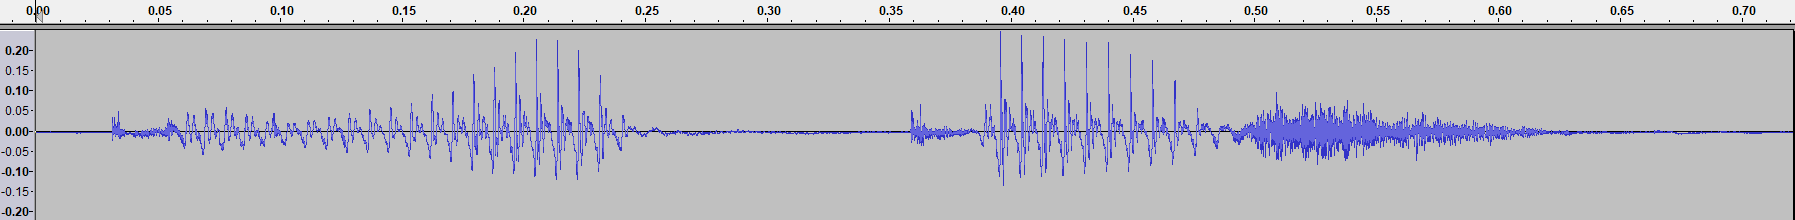
\includegraphics[width=1.0\textwidth]{ex_wave.png}
	\end{figure}
	\begin{figure}[h]
		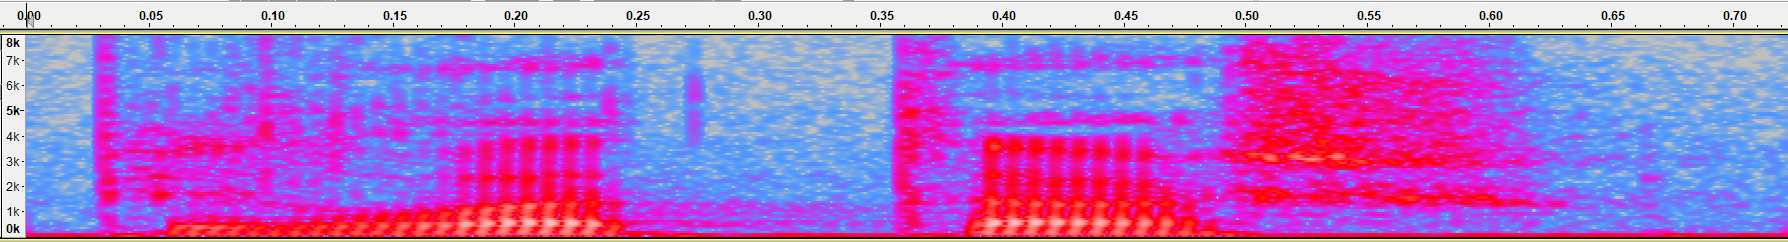
\includegraphics[width=1.0\textwidth]{ex_pp_audacity.png}
	\end{figure}
	\begin{figure}
		\centering
		\begin{minipage}{0.5\textwidth}
			\centering
			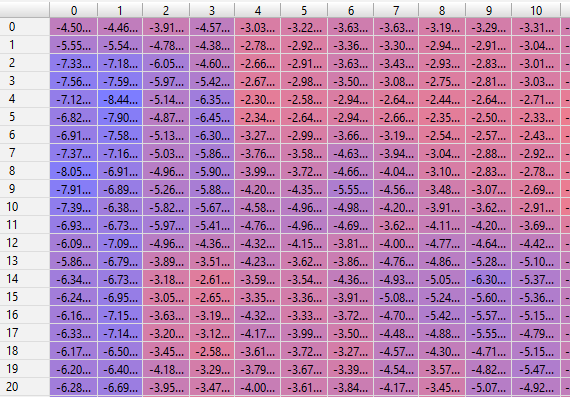
\includegraphics[width=0.83\textwidth]{ex_array_my.png}
		\end{minipage}\hfill
		\begin{minipage}{0.5\textwidth}
			\centering
			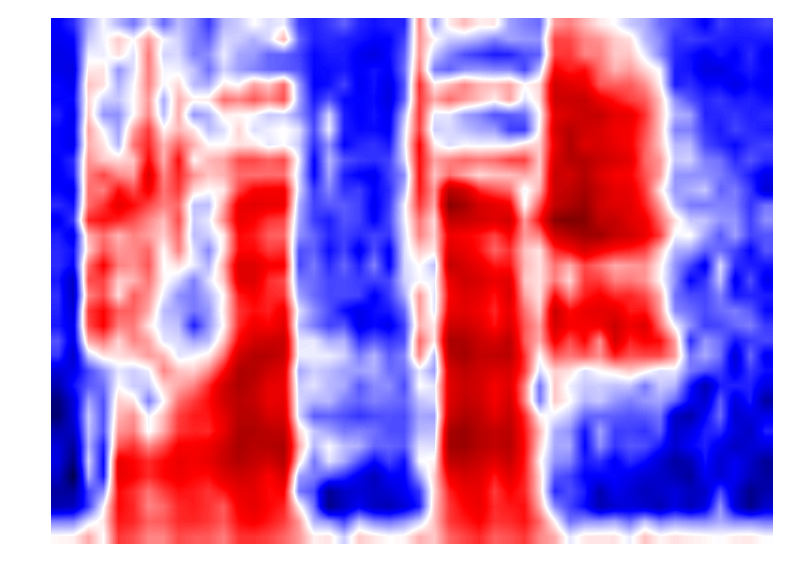
\includegraphics[width=0.88\textwidth]{ex_pp_my.png}
		\end{minipage}
	\end{figure}
	\vfill
\end{frame}

%%%%%%%%%%%%%%%%%%%%%%%%%%%%%%

\begin{frame}
\frametitle{\small Разбиение слов на фонетически однородные части - функционалы}
\footnotesize
\vfill
\circled{1} {\footnotesize Максимальные значения оценок коэффициентов корреляций, усреднённых внутри каждой части}
$$
\max_{a_0, \dots, a_L} \sum_{k=1}^{L} \frac{1}{A_k} \sum^{a_k}_{i=a_{k-1}+1} \sum^{a_k}_{j=i+1} r_{ij}
\text{, где } A_k = \frac{1}{2} (a_k - a_{k-1})(a_k - a_{k-1} - 1)
$$
\vfill
\circled{2} {\footnotesize Минимальные значения дисперсий оценок коэффициентов корреляций внутри каждой части}
$$
\min_{a_0, \dots, a_L} \sum_{k=1}^{L} \frac{1}{A_k-1} \sum^{a_k}_{i=a_{k-1}+1} \sum^{a_k}_{j=i+1} (r_{ij} - \widehat{M}_k)^2
\text{, где } \widehat{M}_k = \frac{1}{A_k} \sum^{a_k}_{i=a_{k-1}+1} \sum^{a_k}_{j=i+1} r_{ij}
$$
\vfill
\circled{3} {\footnotesize Минимальные значения оценок коэффициентов корреляций для соседних частей}
$$
\min_{a_0, \dots, a_L} \sum_{k=1}^{L-1} \frac{1}{A_{k,k+1}} \sum^{a_k}_{i=a_{k-1}+1} \sum^{a_{k+1}}_{j=a_k+1} r_{ij}
\text{, где } A_{k,k+1} = (a_k - a_{k-1})(a_{k+1} - a_k)
$$
\vfill
Итоговый функционал --- это нормированная сумма выражений 1--3
\vfill
\end{frame}

\begin{frame}
\frametitle{\normalsize Стандартная схема динамического программирования}
\footnotesize
\vfill
\begin{figure}[h]
	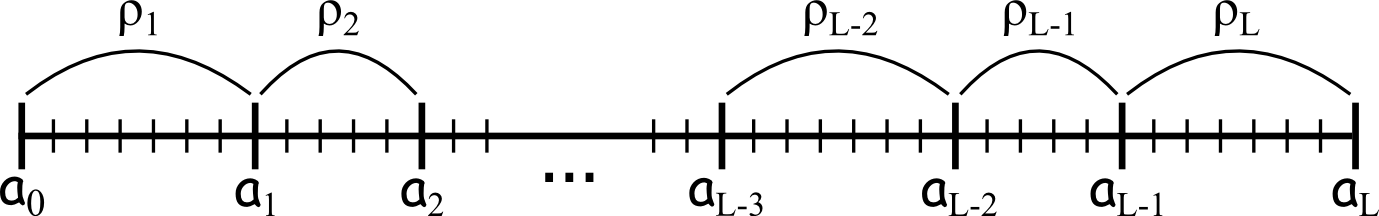
\includegraphics[width=0.9\textwidth]{dinprog_default.png}
\end{figure}
\vfill
$\rho_{k}$ --- оценка среднего коэффициента корреляции внутри части
\bigbreak
Узел $a_L$ фиксирован
\bigbreak
Узлу $a_{L-1}$ задаются приращения $a_{L-1}^j$, $j = \overline{-m, m}$ --- всего $2m+1$ значений \\
Для каждого приращения $a_{L-1}^j$ вычисляется $\rho_L^j$ на участке $[a_{L-1}^j + 1; a_L]$
\bigbreak
Узлу $a_{L-2}$ задаются приращения $a_{L-2}^j$, $j = \overline{-m, m}$ --- также $2m+1$ значений \\
Для каждой $[a_{L-2}^j + 1; a_{L-1}^i]$ вычисляются $\rho_{L-1}^{j, i}$ --- всего $(2m + 1)^2$ значений \\
Максимизируем функционал по правой границе: $P_{L-1}^j = \max_{i} \{\rho_{L-1}^{j, i} + \rho_L^i \}$
\bigbreak
Повторяем вплоть до узла $a_1$, где выбираем итоговый максимум:
$$
P_1 = \max_{j} \{\rho_1^j + P_2^j \}
$$
\vfill
\end{frame}

\begin{frame}
\frametitle{\small Модифицированная схема динамического программирования}
\footnotesize
\vfill
\begin{figure}[h]
	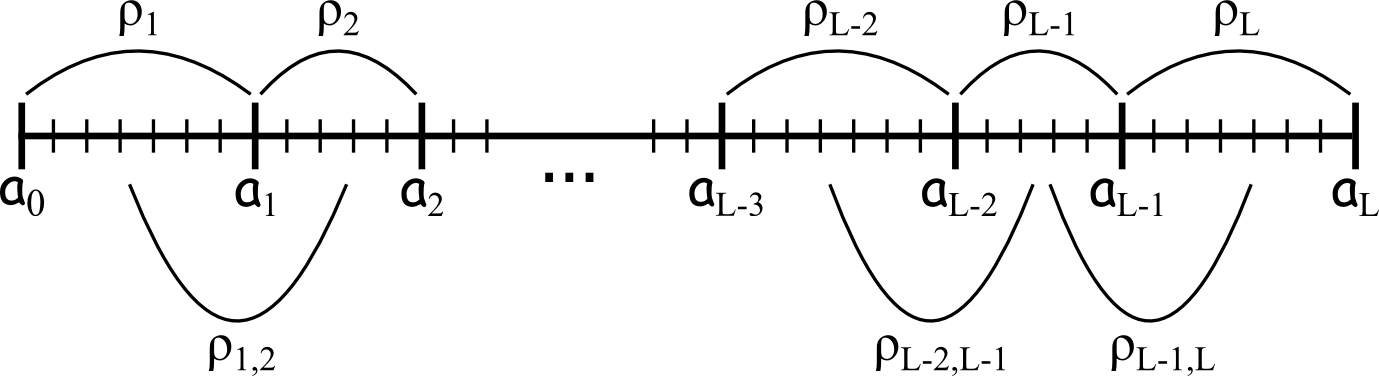
\includegraphics[width=0.9\textwidth]{dinprog_modified.png}
\end{figure}
\vfill
Узлу $a_{L-3}$ задаются приращения $a_{L-3}^j$, $j = \overline{-m, m}$ --- всего $2m+1$ значений \\
Для каждых вариантов частей $[a_{L-3}^j + 1; a_{L-2}^i]$ и $[a_{L-2}^i + 1; a_{L-1}^l]$ вычисляются $\rho_{L-1,L-2}^{l, j, i}$ --- всего $(2m + 1)^3$ значений \\
Максимизируем функционал по 2 правым границам:
$$
P_{L-2, L-1}^{l, j, i} = \rho_{L-2, L-1}^{l, j, i} + P_{L-1, L}^{j, i}
$$
\bigbreak
Остальные шаги проводятся аналогично
\vfill
\end{frame}

\begin{frame}
\frametitle{\small Разбиение слов на фонетически однородные части - примеры}
\footnotesize
\vfill
Слово <<двадцать>>:
\begin{figure}[h]
	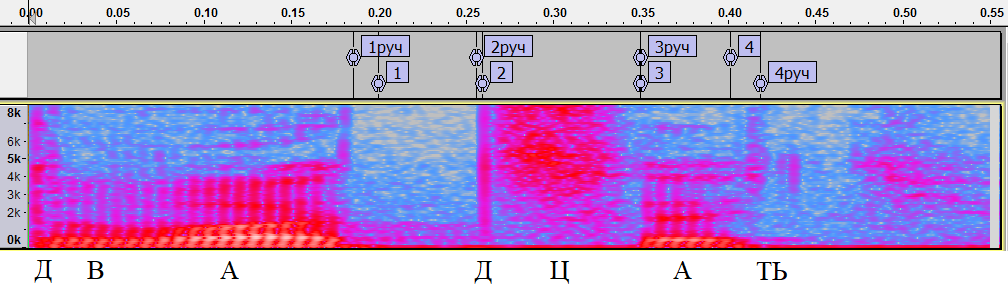
\includegraphics[width=0.88\textwidth]{word_20.png}
\end{figure}
\vfill
Слово <<тысяча>>:
\begin{figure}[h]
	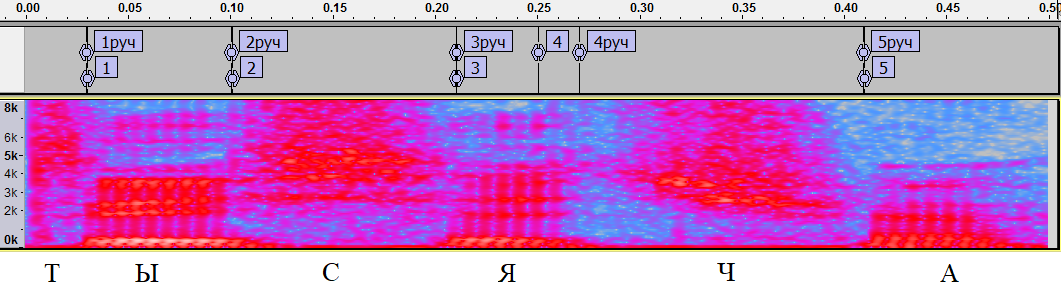
\includegraphics[width=0.88\textwidth]{word_1000.png}
\end{figure}
\vfill
\end{frame}

\begin{frame}
\frametitle{\small Формирование эталонов с помощью метода главных компонент}
\small
\vfill
\begin{itemize}
	\item Переходим к вектору, соединяя временные столбцы
	\item Представим эталоны как $E_{syn} = k_0 a_0 + k_1 a_1 + \dots + k_6 a_6$
	\item Нужно подстроить $k_0, \dots, k_6$ так, чтобы $F \rightarrow \max$
	\item Оптимизация параметров методом покоординатного спуска
\end{itemize}
\vfill
Минимизируемый функционал: $F = \Delta Z^{*low}_{1} + \Delta Z^{*low}_{2} + \Delta Z^{*low}_{3}$,
$$
\text{где }
\Delta Z^{*low}_{i} = \left\{
\begin{array}{ll}
\Delta Z^{low}_{i}, \qquad\qquad\qquad\quad \Delta Z^{low}_{i} \ge 0,\\
\Delta Z^{low}_{i} - \alpha (\Delta Z^{low}_{i})^2, \;\quad \Delta Z^{low}_{i} < 0
\end{array}
\right.
$$

$\Delta Z^{*low}_{i}$ вводит штраф за неправильное распознавание

$$
\Delta Z^{low}_{i} = \min(\Delta Z_{ij}, \Delta Z_{ik}), \qquad i \ne j, i \ne k, j \ne k
$$

где $\Delta Z_{ij} = Z_i - Z_j$, $i$ --- истинное распознаваемое слово,

а $Z = \frac{1}{2} \ln \frac{1 + r}{1 - r}$ --- Z-преобразование Фишера
\vfill
\end{frame}

\begin{frame}
\frametitle{\small Формирование эталонов с помощью метода главных компонент}
\scriptsize
\vfill
Распознавалось 1200 записей, число ошибок снизилось с 60 до 15 или с 5~\% до 1.25~\%.
C шумом в наушниках 80 дБ на обычном (1) и оптимизированном (2) эталонах и \\
с шумом в наушниках 90 дБ на обычном (3) и оптимизированном (4) эталонах.
\footnotesize
\vfill
\begin{table}[h]
	\centering
	\begin{tabular}{| c | c | c | c | c | c |}
		\hline
		\multicolumn{6}{|c|}{Количество ошибок распознавания} \\
		\hline
		Диктор & Слово & \phantom{00} (1) \phantom{00} & \phantom{00} (2) \phantom{00} & \phantom{00} (3) \phantom{00} & \phantom{00} (4) \phantom{00} \\
		\hline
				& пилотаж	& 6 & 0 & 7 & 0 \\
		Б-ак	& масштаб	& 0 & 0 & 0 & 0 \\
				& навигация & 0 & 8 & 0 & 1 \\
		\hline
				& пилотаж	& 3 & 0 & 3 & 0 \\
		Г-ов	& масштаб   & 0 & 0 & 0 & 0 \\
				& навигация & 0 & 0 & 0 & 2 \\
		\hline
				& пилотаж	& 8 & 0 & 12& 0 \\
		Н-ов	& масштаб   & 0 & 0 & 0 & 0 \\
				& навигация & 0 & 0 & 0 & 0 \\
		\hline
				& пилотаж	& 9 & 0 & 4 & 0 \\
		Ф-ев	& масштаб   & 0 & 0 & 0 & 0 \\
				& навигация & 0 & 0 & 8 & 4 \\
		\hline
		\multicolumn{2}{|c|}{Суммарные результаты} & \multicolumn{2}{c|}{$26 \quad\longrightarrow\quad 8$} & \multicolumn{2}{c|}{$34 \quad\longrightarrow\quad 7$} \\
		\hline
	\end{tabular}
\end{table}
\vfill
\end{frame}

\begin{frame}
\frametitle{\small Формирование эталонов с помощью метода главных компонент}
\footnotesize
\vfill
Определение оптимального (по функционалу $F$) числа реализаций команд и количества итераций в процессе оптимизации коэффициентов
\vfill
\begin{table}[h]
	\centering
	{\scriptsize
		\begin{tabular}{ l | l | C | C | C || C | C | C |}
			\cline{2-8}
			& Реализации& \multicolumn{3}{c||}{1}  & \multicolumn{3}{c|}{10} \\
			\cline{2-8}
			& Итерации 	& 0 & 3 & 10  	   & 0 & 3 & 10  \\
			\hline
			\multicolumn{1}{|c|}{Диктор}& Слово 	& \multicolumn{6}{c|}{Число ошибок}	\\
			\hline
			\multicolumn{1}{|c|}{}		& пилотаж 	& 0  & 0  & 0    & 0  & 0  & 0  \\
			\multicolumn{1}{|c|}{К-ов}	& масштаб 	& 0  & 0  & 0    & 0  & 0  & 0  \\
			\multicolumn{1}{|c|}{}		& навигация & 7  & 0  & 0    & 7  & 0  & 0  \\
			\hline
			\multicolumn{1}{|c|}{}		& пилотаж 	& 0  & 0  & 0    & 0  & 0  & 0  \\
			\multicolumn{1}{|c|}{О-ин}	& масштаб 	& 0  & 0  & 0    & 0  & 0  & 0  \\
			\multicolumn{1}{|c|}{}		& навигация & 0  & 0  & 0    & 0  & 0  & 0  \\
			\hline
			\multicolumn{1}{|c|}{}		& пилотаж 	& 0  & 0  & 0    & 0  & 0  & 0  \\
			\multicolumn{1}{|c|}{С-ев}	& масштаб 	& 6  & 0  & 0    & 6  & 1  & 0  \\
			\multicolumn{1}{|c|}{}		& навигация & 0  & 1  & 1    & 0  & 1  & 1  \\
			\hline
			\multicolumn{1}{|c|}{}		& пилотаж 	& 1  & 1  & 1    & 1  & 1  & 1  \\
			\multicolumn{1}{|c|}{Ц-ин} 	& масштаб 	& 0  & 0  & 0    & 0  & 0  & 0  \\
			\multicolumn{1}{|c|}{}		& навигация & 0  & 0  & 0    & 0  & 0  & 0  \\
			\hline
		\end{tabular}
	}
\end{table}
\vfill
Вывод: для оптимизации коэффициентов достаточно всего \\
$\qquad\quad$ \textbf{1} записи в обучающей выборке и \textbf{10} итераций
\vfill
\end{frame}

\begin{frame}
\frametitle{\small Сжатие параметрических портретов полиномами Чебышёва}
\small
Цель: уменьшить размер параметрического портрета, чтобы ускорить его обработку 
\bigbreak
Решаем стандартную задачу аппроксимации:
$$
S_m = \sum_{i=0}^{n} \left[Q_m (x_i) - f(x_i) \right]^2 \rightarrow \min_{Q_m (x)} ,\quad m - \text{степень полинома,}
$$
а $f(x_i)$ --- строка или столбец параметрического портрета.
\vfill
2 способа задания вычисления полиномов Чебышёва 1-го рода:
\begin{columns}
	\begin{column}{0.5\textwidth}
		$$
		T_n (x) = \sum_{k=0}^{\lfloor n/2 \rfloor} \binom{n}{2k} (x^2 - 1)^k x^{n-2k}
		$$
	\end{column}
	\begin{column}{0.5\textwidth}
		$$
		\begin{gathered}
		T_0 (x) = 1 \\
		T_1 (x) = x \\
		%T_2 (x) = 2x^2 - 1 \\
		\vdots \\
		T_{n+1} (x) = 2x T_n (x) - T_{n-1} (x)
		\end{gathered}
		$$
	\end{column}
\end{columns}

\end{frame}

\begin{frame}
\frametitle{\small Сжатие параметрических портретов полиномами Чебышёва}
\footnotesize
\vfill
Цель: снижение размерности параметрических портретов с сохранением качества распознавания
\vfill
Изначальный портрет размером $35 \times 48$ имел \textbf{1.6~\%} ошибок \\
Сжатый портрет: до $18 \times 18$ даёт \textbf{1.8~\%} ошибок, а до $12 \times 12$ - \textbf{2.0~\%} ошибок
\vfill
\begin{figure}[h]
	\centering
	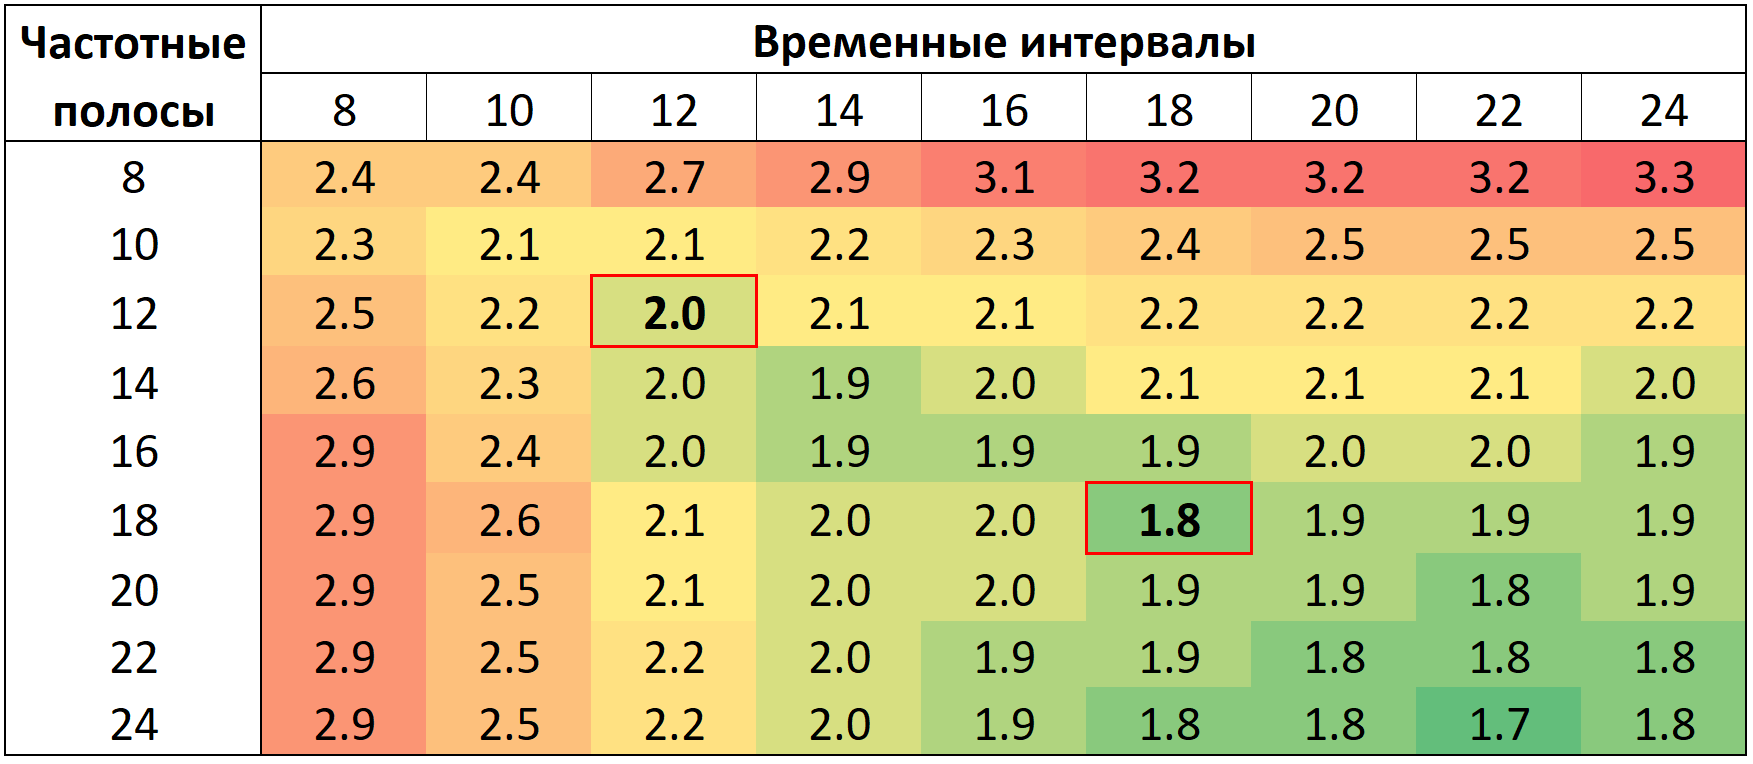
\includegraphics[width=1.0\textwidth]{chebyshev.png}
\end{figure}
\vfill
\end{frame}

\begin{frame}
\frametitle{\normalsize Распознавание несколькими эталонами - метод Байеса}
\small
\vfill
Гипотеза $H_i$: истинное слово - это слово $i$ \\
Событие $A_k$: распознанное слово - это слово $k$ \\
$M$ - общее количество слов в словаре \\
\bigbreak
% Стандартная формула Байеса: $$P(H_i|A_k) = \frac{P(H_i) P(A_k|H_i)}{\sum_{i=1}^M P(H_i) P(A_k|H_i)}$$

Модифицированная формула Байеса для $L$ эталонов:
$$
P(H_i|A_{k_1 k_2 \dots k_L}) =
\frac{P(H_i) P(A_{k_1 k_2 \dots k_L}|H_i)}{\sum_{i=1}^M P(H_i) P(A_{k_1 k_2 \dots k_L}|H_i)}
$$
{\footnotesize
$P(H_1) = \dots = P(H_M) = \frac{1}{M}, \quad P(A_{k_1 k_2 \dots k_L}|H_i)$ --- из обучающей выборки
}
\vfill
В нашем случаи эталоны независимы, поэтому:
$$
A_{k_1 k_2 \dots k_L} = A_{k_1}^{C_1} A_{k_2}^{C_2} \dots A_{k_L}^{C_L} \text{, где } C_i \text{ - соответствущий эталон}
$$
\end{frame}

\begin{frame}
\frametitle{\normalsize Распознавание несколькими эталонами - метод Байеса}
\footnotesize
\vfill
Тогда выражение для условных вероятностей принимает вид:
$$
P(A_{k_1 k_2 \dots k_L}|H_i) = P(A_{k_1}^{C_1}|H_i) P(A_{k_2}^{C_2}|H_i) \dots P(A_{k_L}^{C_L}|H_i) = \prod_{j=1}^{L} P(A_{k_j}^{C_j}|H_i)
$$
\vfill
Введём учёт качества распознавания: 

$$
\Delta Z^j = Z_{\max}^j - Z_{\max-1}^j,\quad
P(A_k^{\Delta Z}|H_i) = P(A_k \cap \Delta Z|H_i) = P(A_k|H_i) P(\Delta Z|H_i)
$$

$Z = \frac{1}{2} \ln \frac{1 + r}{1 - r}$ --- Z-преобразование Фишера

% $$P_c(\Delta Z_j|H_i) = \frac{n_c^i(\Delta Z_j)}{n_c^i(\Delta Z_j) + n_{nc}^i(\Delta Z_j)},\quad P_{nc}(\Delta Z_j|H_i) = \frac{n_{nc}^i(\Delta Z_j)}{n_c^i(\Delta Z_j) + n_{nc}^i(\Delta Z_j)}$$
% $$P(\Delta Z|H_i) = P_c(\Delta Z|H_i), \text{ если } i=k, \text{ и } P(\Delta Z|H_i) = P_{nc}(\Delta Z|H_i), \text{ если } i \ne k$$
\vfill
Итоговое выражение:
$$
P(H_i|A_{k_1 k_2 \dots k_L}^{\Delta Z^1 \Delta Z^2 \dots \Delta Z^L}) = 
\frac{P(H_i) \prod_{j=1}^{L} P(A_{k_j}^{C^j}|H_i) P^{C^j}(\Delta Z^j|H_i)}{\sum_{i=1}^M P(H_i) \prod_{j=1}^{L} P(A_{k_j}^{C^j}|H_i) P^{C^j}(\Delta Z^j|H_i)}
$$
\vfill
\end{frame}

\begin{frame}
\frametitle{\small Распознавание несколькими эталонами - метод комитетов}
{\small Результатом распознавания принимается слово, за которое <<проголосовало>> большинство <<членов комитета>>}
\noindent\makebox[\linewidth]{\rule{0.9\paperwidth}{0.6pt}}
Суммарный рейтинг $R_i$ по $L$ эталонам:
$$
R_i = \sum_{j=1}^L r_i^j = \sum_{j=1}^L \frac{Z_i^j}{p_i^j} \Delta Z^j,
$$
где~$j$~-~номер~эталона,~$i$~-~номер~субэталона,
\phantom{где}~$p_i^j$~-~позиция~субэталона~в~рейтинге,
\phantom{где}~$Z_i^j$~-~значение~скалярной~меры~близости,
\phantom{где}~$\Delta Z^j = Z_{\max}^j - Z_{\max-1}^j$~-~мера~качества~распознавания
\end{frame}

\begin{frame}
\frametitle{\normalsize Распознавание несколькими эталонами - результаты}
\small
\vfill
Распознавание 7 эталонами из <<чужих>> дикторов
\begin{table}[h]
	\centering
	{\small
		\begin{tabular}{| l | c | c | c | c | c | c | c | c | c |}
			\hline
			\multicolumn{10}{|c|}{\textbf{Процент ошибок распознавания}} \\
			\hline
			Вариант & \multicolumn{8}{c|}{Порядковый номер диктора} & Среднее \\
			\hhline{~--------}
			теста & 1 & 2 & 3 & 4 & 5 & 6 & 7 & 8 & значение \\
			\hline
			\hline
			1 эталон	& 5.3 & 9.3 & 15  & 8.0 & 5.0 & 11  & 7.0 & 6.7 & \textbf{8.4} \\
			\hline
			\multicolumn{10}{|c|}{алгоритм на основе формулы Байеса} \\
			\hline
			до 1 слова	& 4.8 & 7.3 & 7.3 & 4.8 & 6.5 & 6.3 & 4.7 & 3.2 & \textbf{5.6} \\
			до 2 слов	& 2.7 & 4.8 & 3.8 & 2.2 & 2.5 & 2.7 & 2.2 & 0.8 & 2.7 \\
			до 3 слов	& 2.5 & 3.5 & 3.0 & 1.8 & 2.2 & 2.2 & 2.0 & 0.7 & 2.2 \\
			\hline
			\multicolumn{10}{|c|}{алгоритм на основе метода комитетов} \\
			\hline
			до 1 слова	& 4.5 & 7.3 & 7.2 & 4.8 & 4.5 & 6.7 & 4.8 & 2.8 & \textbf{5.3} \\
			до 2 слов	& 0.7 & 3.3 & 2.8 & 1.3 & 1.7 & 2.7 & 1.0 & 1.3 & 1.9 \\
			до 3 слов	& 0.5 & 2.5 & 1.0 & 0.5 & 1.3 & 1.7 & 0.5 & 0.5 & 1.1 \\
			\hline
			подстройка	& 1.8 & 4.5 & 4.3 & 3.2 & 1.9 & 4.8 & 2.3 & 2.2 & \textbf{3.1} \\
			\hline
		\end{tabular}
	}
\end{table}
\vfill
\end{frame}

%%%%%%%%%%%%%%%%%%%%%%%%%%%%%%

\begin{frame}
\frametitle{\normalsize Распознавание свёрточными нейронными сетями}
Структура используемой свёрточной нейронной сети
\begin{figure}[h]
	\centering
	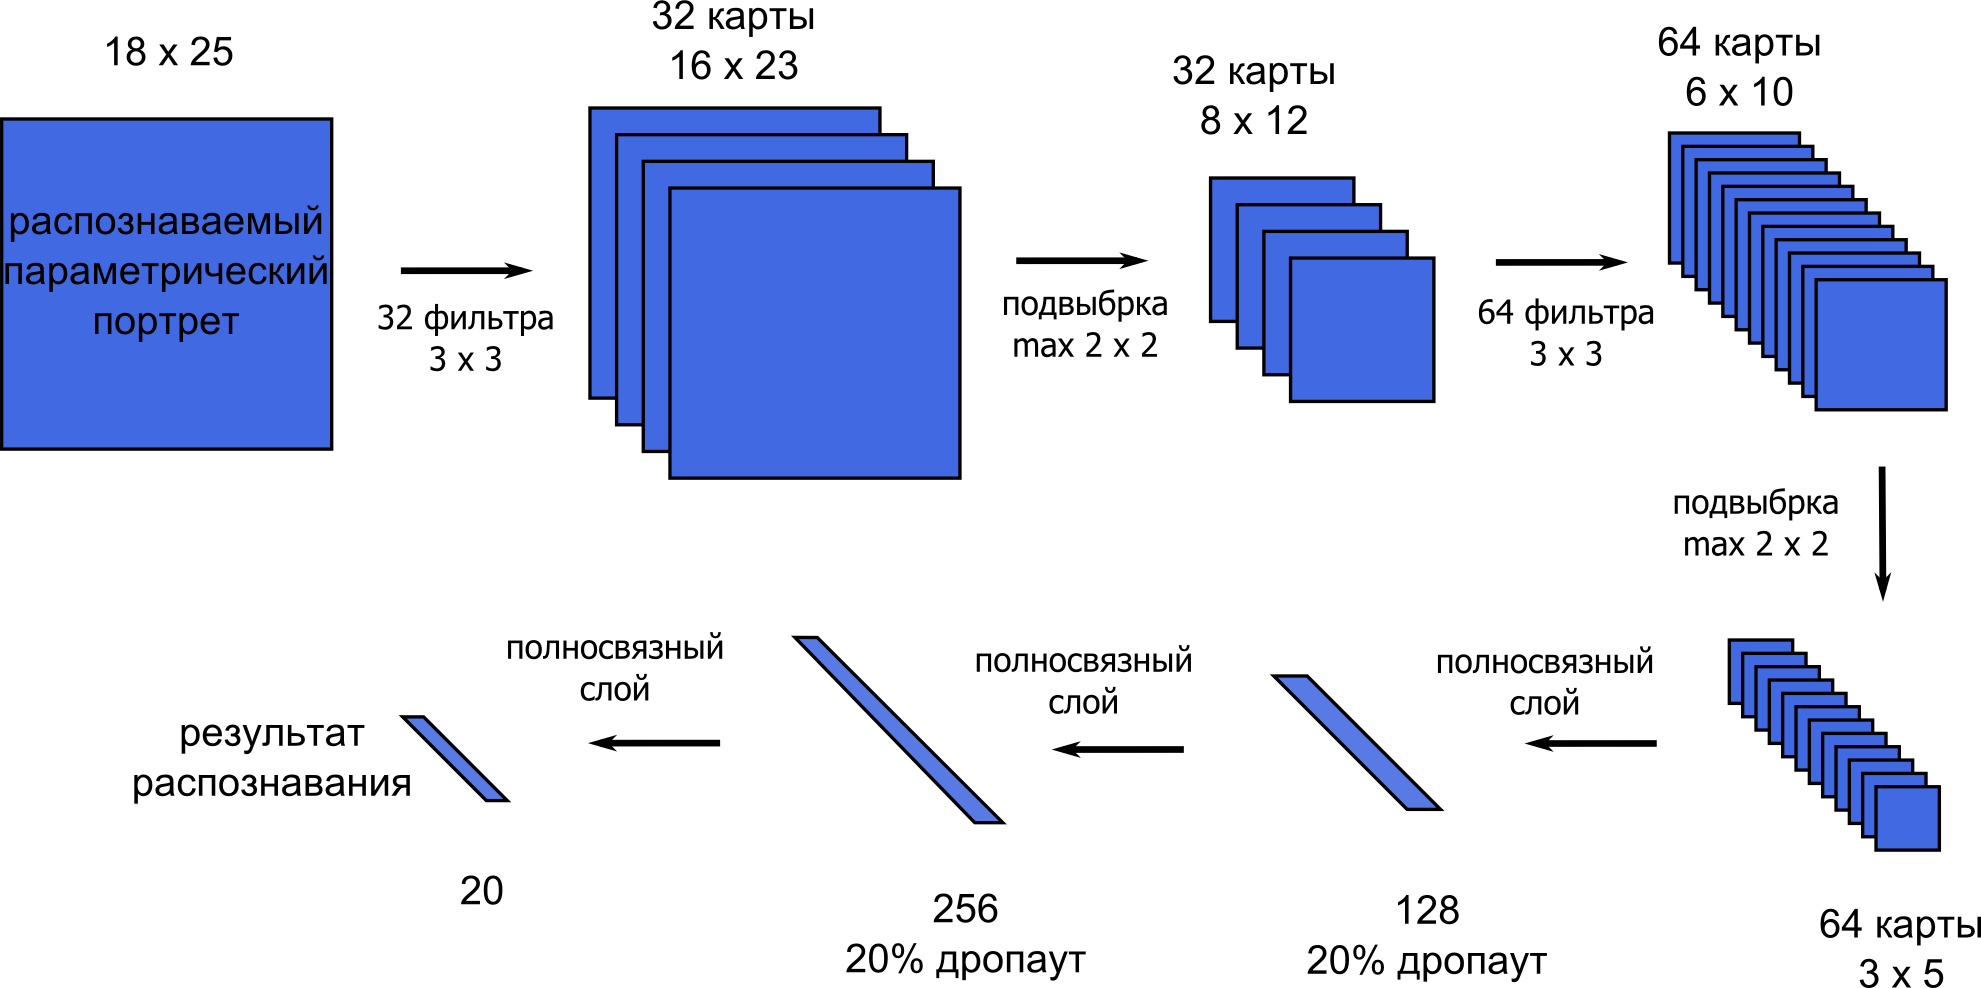
\includegraphics[width=1.0\textwidth]{cnn_my.png}
\end{figure}
\end{frame}

\begin{frame}
\frametitle{\normalsize Свёрточные нейронные сети - распознавание без шума}
\footnotesize
\vfill
Суммарные результаты при распознавании команд без шума
\vfill
\begin{figure}[h]
	\centering
	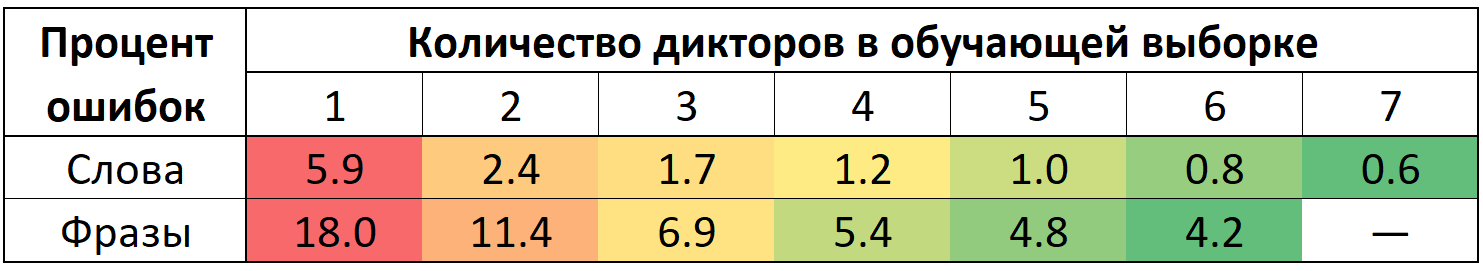
\includegraphics[width=0.92\textwidth]{cnn_total.png}
\end{figure}
\vfill
Распознавание фраз по <<чужому>> диктору с добавлением <<своего>> диктора
\vfill
\begin{figure}[h]
	\centering
	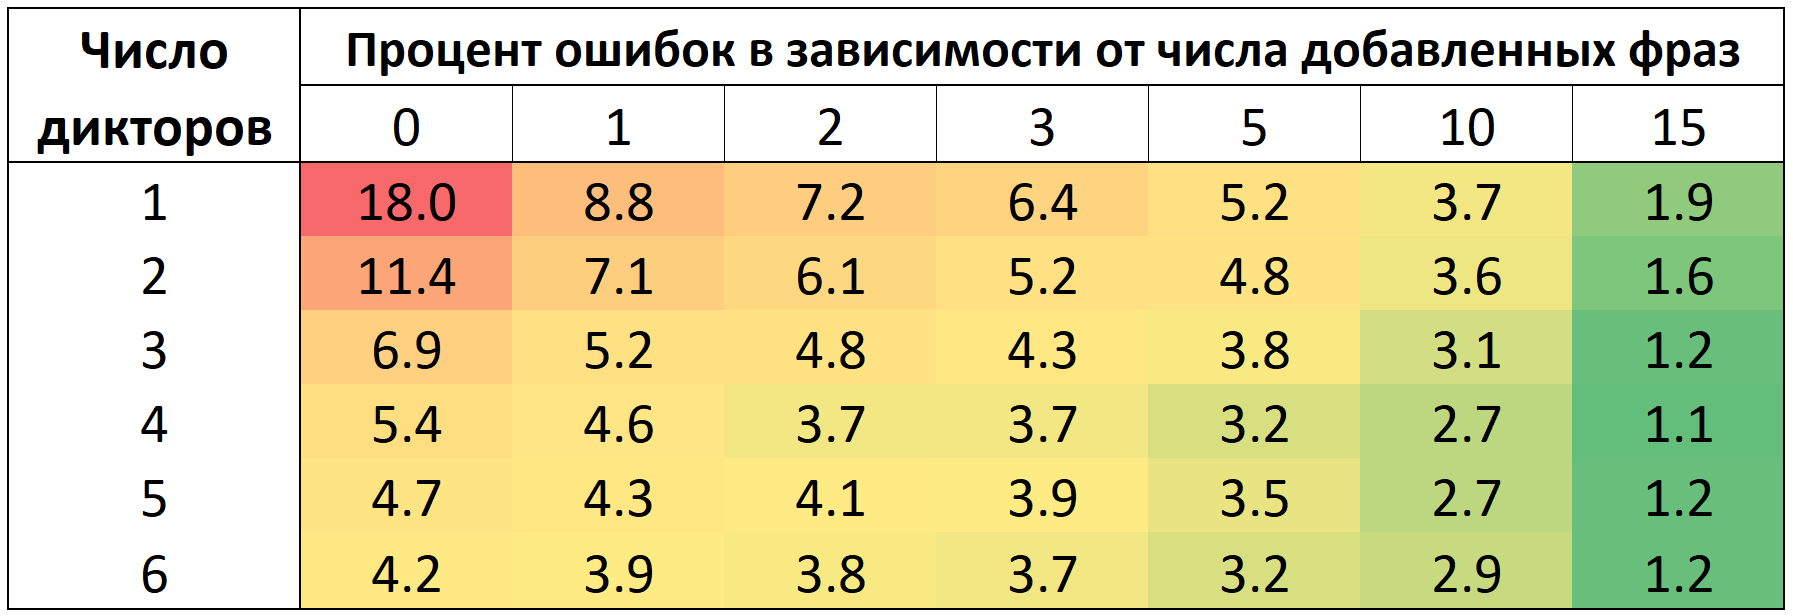
\includegraphics[width=0.92\textwidth]{cnn_additional.png}
\end{figure}
\vfill
\end{frame}

\begin{frame}
\frametitle{\normalsize Свёрточные нейронные сети - распознавание с шумом}
\footnotesize
\vfill
\begin{table}[h]
	\centering
	\begin{tabular}{| l | c || c | c |}
		\hline
		\multicolumn{2}{|c||}{Обучающая выборка}	& \multicolumn{2}{c|}{Процент ошибок}	\\
		\hline
		число			& число шумов			 	& обучающая & тестовая	\\
		дикторов		& \textbf{SNR = 6 дБ}		& выборка 	& выборка	\\
		\hline
		\multicolumn{4}{|c|}{\textbf{слова}} \\
		\hline
		\multirow{2}{*}{1 диктор}	& 1				& 0.3 		& 9.7  		\\
		\hhline{~---}
		& 7				& 0.0 		& 8.2  		\\
		\hline
		\multirow{2}{*}{3 диктора}	& 1				& 0.0 		& 2.8  		\\
		\hhline{~---}
		& 3				& 0.0 		& 2.5  		\\
		\hline
		\multirow{2}{*}{7 дикторов}	& 1				& 0.0 		& 1.2  		\\
		\hhline{~---}
		& 3				& 0.0 		& \textbf{1.1}  		\\
		\hline
		\multicolumn{4}{|c|}{\textbf{фразы}} \\
		\hline
		\multirow{2}{*}{1 диктор}	& 1				& 0.0 		& 22.4  	\\
		\hhline{~---}
		& 10			& 0.0 		& 20.8  	\\
		\hline
		\multirow{2}{*}{3 диктора}	& 1				& 0.0 		& 11.5  	\\
		\hhline{~---}
		& 5				& 0.0 		& 10.4  	\\
		\hline
		\multirow{2}{*}{6 дикторов}	& 1				& 0.0 		& 8.4  		\\
		\hhline{~---}
		& 2				& 0.0 		& \textbf{7.0}  		\\
		\hline
	\end{tabular}
\end{table}
\vfill
\end{frame}

\begin{frame}
\frametitle{\normalsize Свёрточные нейронные сети - распознавание по себе}
\small
\vfill
Выборка из 30 записей каждой команды разбивается на 2 части: обучающую для подбора весов и тестовую для распознавания
\vfill
\begin{figure}[h]
\centering
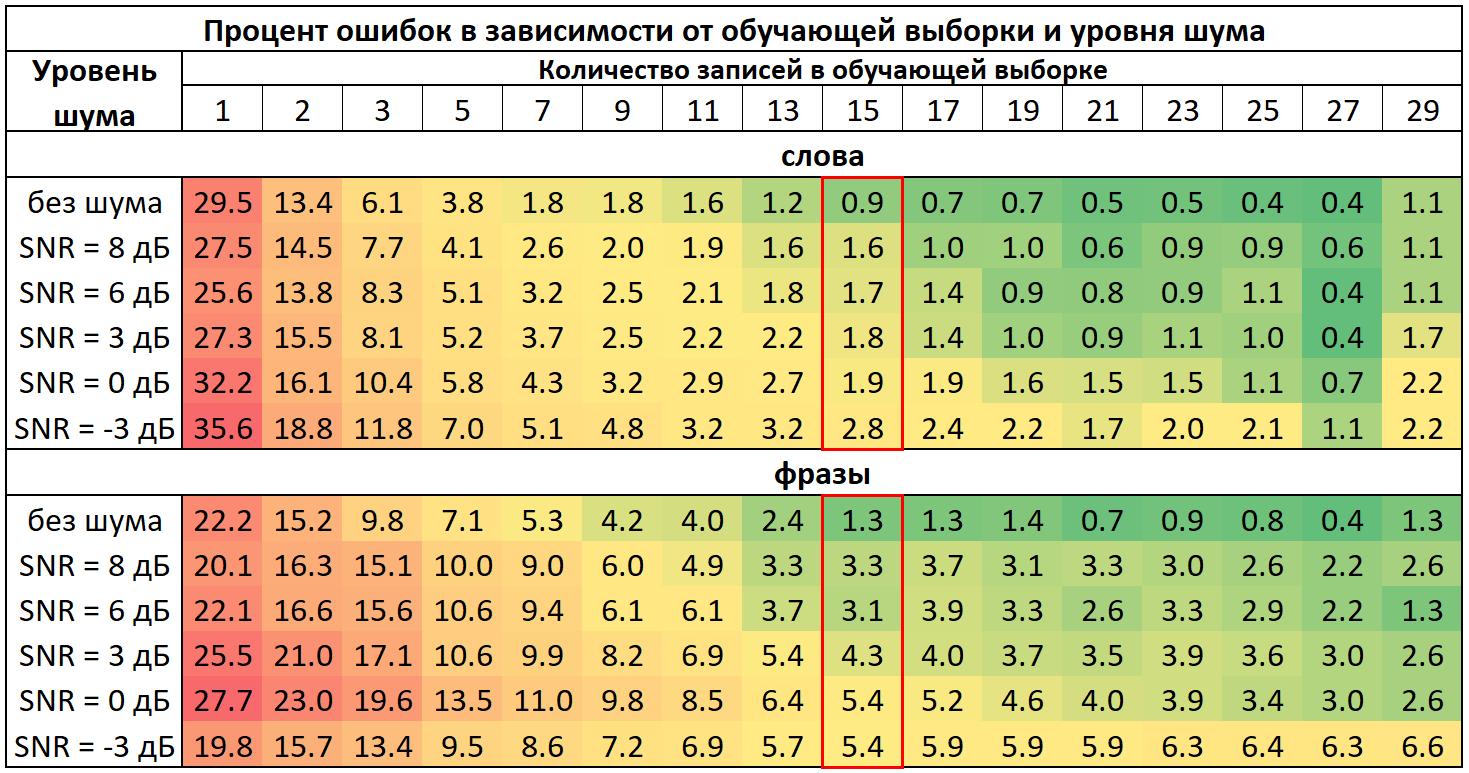
\includegraphics[width=1.0\textwidth]{cnn_self_noise.png}
\end{figure}
\vfill
\end{frame}

%%%%%%%%%%%%%%%%%%%%%%%%%%%%%%

\begin{frame}
\frametitle{\large Результаты работы - сравнение с эталоном}
\small
\vfill
Предложен ряд новых алгоритмов:
\footnotesize
\vfill
\begin{enumerate}
	\item Автоматического разбиения слов на однородные участки на основе модифицированного метода динамического программирования --- уменьшает долю ошибок с~\textbf{5.3}~до~\textbf{3.1~\%} при распознавании 20 слов алгоритмом на основе метода комитетов
	\item Улучшения качества эталона, основанный на выделении и оптимизации главных компонент --- уменьшает долю ошибок с~\textbf{5}~до~\textbf{1.25~\%} при распознавании 3 слов
	\item Сжатия параметрического портрета с помощью применения полиномов Чебышёва --- сокращает место для хранения информации в~\textbf{5--10} раз и существенно улучшает быстродействие алгоритмов распознавания
	\item Распознавания несколькими эталонами на основе формулы Байеса --- уменьшает процент ошибок с~\textbf{8.4}~до~\textbf{5.6~\%} при распознавании 20 слов, а на основе метода комитетов --- до \textbf{5.3~\%}
\end{enumerate}
\vfill
\end{frame}

\begin{frame}
\frametitle{Результаты работы - нейронные сети}
\small
\vfill
Предложенные алгоритмы на основе свёрточных нейронных сетей показал следующие результаты:
\footnotesize
\vfill
\begin{enumerate}
	\item Процент ошибок распознавания для \underline{слов} составляет \textbf{0.6~\%} в условиях без шума и \textbf{1.1~\%} для отношения сигнал/шум 6 дБ
	\item Процент ошибок распознавания для \underline{фраз} составляет \textbf{4.2~\%} в условиях без шума и \textbf{7.0~\%} для отношения сигнал/шум 6 дБ
	\item Обучение на 15 \underline{словах} <<своего>> диктора даёт \textbf{0.9~\%} в условиях без шума и \textbf{1.7~\%} для отношения сигнал/шум 6 дБ
	\item Обучение на 15 \underline{фразах} <<своего>> диктора даёт \textbf{1.3~\%} в условиях без шума и \textbf{3.1~\%} для отношения сигнал/шум 6 дБ
	\item Значительное снижение процента ошибок при дополнительном обучении на нескольких записях \underline{фраз} <<своего>> диктора
\end{enumerate}
\vfill
\end{frame}

\begin{frame}
	\begin{center}
		\large
		\vfill	
		Доклад окончен.
		\vfill	
		Спасибо за внимание!
		\vfill
	\end{center}
\end{frame}

%%%%%%%%%%%%%%%%%%%%%%%%%%%%%%

%\begin{frame}[noframenumbering]
% 
%\end{frame}
%
%\begin{frame}[noframenumbering]
%\frametitle{\large Результаты работы - сравнение с эталоном}
%\small
%\vfill
%Предложен ряд новых алгоритмов:
%\footnotesize
%\vfill
%\begin{enumerate}
%	\item Автоматического разбиения слов на однородные участки на основе модифицированного метода динамического программирования --- уменьшает долю ошибок с~\textbf{5.3~(1.5)}~до~\textbf{3.1~(1.2)~\%} при распознавании 20 слов алгоритмом на основе метода комитетов
%	\item Улучшения качества эталона, основанный на выделении и оптимизации главных компонент --- уменьшает долю ошибок с~\textbf{5~(2.1)}~до~\textbf{1.25~(1.7)~\%} при распознавании 3 слов
%	\item Сжатия параметрического портрета с помощью применения полиномов Чебышёва --- сокращает место для хранения информации в~\textbf{5--10} раз и существенно улучшает быстродействие алгоритмов распознавания
%	\item Распознавания несколькими эталонами на основе формулы Байеса --- уменьшает процент ошибок с~\textbf{8.4~(3.2)}~до~\textbf{5.6~(1.4)~\%} при распознавании 20 слов, а на основе метода комитетов --- до \textbf{5.3~(1.5)~\%}
%\end{enumerate}
%\vfill
%\end{frame}
%
%\begin{frame}[noframenumbering]
%\frametitle{Результаты работы - нейронные сети}
%\small
%\vfill
%Предложенные алгоритмы на основе свёрточных нейронных сетей показал следующие результаты:
%\footnotesize
%\vfill
%\begin{enumerate}
%	\item Процент ошибок распознавания для \underline{слов} составляет \textbf{0.6~(0.4)~\%} в условиях без шума и \textbf{1.1~(0.8)~\%} для отношения сигнал/шум 6 дБ
%	\item Процент ошибок распознавания для \underline{фраз} составляет \textbf{4.2~(3.2)~\%} в условиях без шума и \textbf{7.0~(4.3)~\%} для отношения сигнал/шум 6 дБ
%	\item Обучение на 15 \underline{словах} <<своего>> диктора даёт \textbf{0.9~(0.5)~\%} в условиях без шума и \textbf{1.7~(0.8)~\%} для отношения сигнал/шум 6 дБ
%	\item Обучение на 15 \underline{фразах} <<своего>> диктора даёт \textbf{1.3~(1.6)~\%} в условиях без шума и \textbf{3.1~(3.5)~\%} для отношения сигнал/шум 6 дБ
%	\item Значительное снижение процента ошибок при дополнительном обучении на нескольких записях \underline{фраз} <<своего>> диктора
%\end{enumerate}
%\vfill
%\end{frame}